% !TEX root = ../../main.tex
\chapter{Reconstructing Neutrino $p_z$}
\label{ch:neutrinopz}

Along the beam axis, $\hat{z}$, an unknown fraction of energy from the event escapes. This restricts the ability to constrain missing energy to the transverse $\hat{x}-\hat{y}$ plane, as described in \Ch{\ref{ch:objreco}}. 
For the event topology of this analysis, $WV\to l\nu J$, the neutrino escapes the detector leaving virtually no energy deposit; thus, the missing energy in the transverse plane, $E_{\mathrm T}^{\rm miss}$, is attributed to the transverse momentum of the neutrino, $p_{\mathrm{T}, \nu}$. The invariant mass of the $WV$ system is given below in \Eqn{\ref{eq:wv_m}}.
\begin{equation}
m_{WV}^2 = \left(E_{J} + E_{l} + E_{\nu}\right)^2 - \left(\vec{p}_{J} + \vec{p}_{l} + \vec{p}_{\nu}\right)^2
\label{eq:wv_m}
\end{equation}

Since only the transverse momentum of the neutrino is known, however, \Eqn{\ref{eq:wv_mt}} for the transverse mass, $m_{\mathrm{T}}$, must be used.
\begin{equation}
m_{\mathrm{T}, WV}^2 = \left(E_{\mathrm{T}, J} + E_{\mathrm{T}, l} + E_{\mathrm{T}, \nu}\right)^2 - \left(\vec{p}_{\mathrm{T}, J} + \vec{p}_{\mathrm{T}, l} + \vec{p}_{\mathrm{T}, \nu}\right)^2
\label{eq:wv_mt}
\end{equation}

The transverse mass, $m_{\mathrm{T}, WV}$, will have a dependence on the angle between the daughter particles, and will have worse resolution than the invariant mass. It would be more desirable to be able to use \Eqn{\ref{eq:wv_m}} to provide a better signal to background ratio.


It is therefore advantageous to reconstruct the $\hat{z}$ component of the neutrino momentum vector, $p_{z,\nu}$, with the constraint of the $W$ boson mass, $m_W$ (80.385\,\GeV). Using energy-momentum 4-vectors, $p^{\mu}=(E, \vec{p})$, for the $W$ boson, lepton, and neutrino, it is possible to derive a quadratic expression for $p_{z,\nu}$ in terms of $m_W$, $\vec{p}_l$, and $p_{\mathrm{T}, \nu}$. 
\begin{eqnarray}
    m_W^2 &=&p_W^{\mu}p_{W,\mu} = (p^{\mu}_l+p^{\mu}_{\nu})(p_{l,\mu}+p_{\nu, \mu}) \nonumber \\
    &=& m_l^2 + m_{\nu}^2 + 2(\Cline[red]{E_l}E_{\nu}-\vec{p}_l\cdot\vec{p}_{\nu}) \label{eq:n_first} \\
    &=& 2\Cline[red]{\sqrt{p_{\mathrm{T},l}^2+p_{z,l}^2}}\sqrt{p_{\mathrm{T},\nu}^2+p_{z, \nu}^2}\nonumber\\
    &&-2\vec{p}_{\mathrm{T},l}\cdot \vec{p}_{\mathrm{T},\nu}-2p_{z,l}p_{z,\nu} \label{eq:n_el}\\
\left(\Cline[green]{m_W^2+2\vec{p}_{\mathrm{T},l}\cdot \vec{p}_{\mathrm{T},\nu}}+2p_{z,l}p_{z,\nu}\right)^2    &=&4(p_{\mathrm{T},l}^2+p_{z,l}^2)(p_{\mathrm{T},\nu}^2+p_{z, \nu}^2) \label{eq:n_c} \\
 \Cline[green]{C}^2 + 4\Cline[green]{C}p_{z,l}p_{z,\nu}+\Cline[blue]{4p_{z,l}^2p_{z,\nu}^2}&=&   4\left[p_{\mathrm{T},l}^2p_{z,\nu}^2+p_{\mathrm{T},\nu}^2(p_{\mathrm{T},l}^2+p_{z,l}^2)+\Cline[blue]{p_{z,l}^2p_{z,\nu}^2}\right] \label{eq:n_cancel}\\
   0&=& \left[4p_{\mathrm{T},l}^2\right]p_{z,\nu}^2 - \left[4Cp_{z,l}\right]p_{z,\nu}+ \nonumber \\ 
   &&\left[4p_{\mathrm{T},\nu}^2(p_{\mathrm{T},l}^2+p_{z,l}^2)-C^2\right] \label{eq:n_final}
\end{eqnarray}

In \Eqn{\ref{eq:n_el}}, the limit where the neutrino mass is negligible is taken. It is also prudent to take the limit where the lepton momentum is much larger than the mass, $m_l$, which drops out as well in \Eqn{\ref{eq:n_el}}. 
The lepton energy, $E_l$, underlined in red in \Eqn{\ref{eq:n_first}} is then approximated to be equal to the magnitude of the lepton momentum, $\vec{p_l}$, underlined in red in \Eqn{\ref{eq:n_el}}. The radical in \Eqn{\ref{eq:n_el}} is removed in \Eqn{\ref{eq:n_c}} by isolating it and squaring both sides. The green underlined quantity in \Eqn{\ref{eq:n_c}} is redefined as a constant, $C$, in  \Eqn{\ref{eq:n_cancel}}. In \Eqn{\ref{eq:n_cancel}}, the blue underlined quantities cancel out, leading to the result in \Eqn{\ref{eq:n_final}} which is a quadratic equation for $p_{z,\nu}$.

There can be up to two solutions in this case for $p_{z,\nu}$, which are handled as follows:
\begin{enumerate}
	\item If a solution is complex, remove the imaginary part
	\item If two unique solutions exist, compare the magnitudes and keep the smallest one
\end{enumerate}

The effect of these choices are minimal, and presented in \Fig{\ref{fig:neutrinoPz}}. In \Fig{\ref{fig:mass_vs_mt}}, the reconstructed invariant mass (using the $p_{z,\nu}$ defined above) is compared to the transverse mass. It is clear that the invariant mass reproduces the signal mass with a sharper peak, smaller width, and more accurate mean value. 

\begin{figure}[hp]
 \begin{center}
\subfloat[]{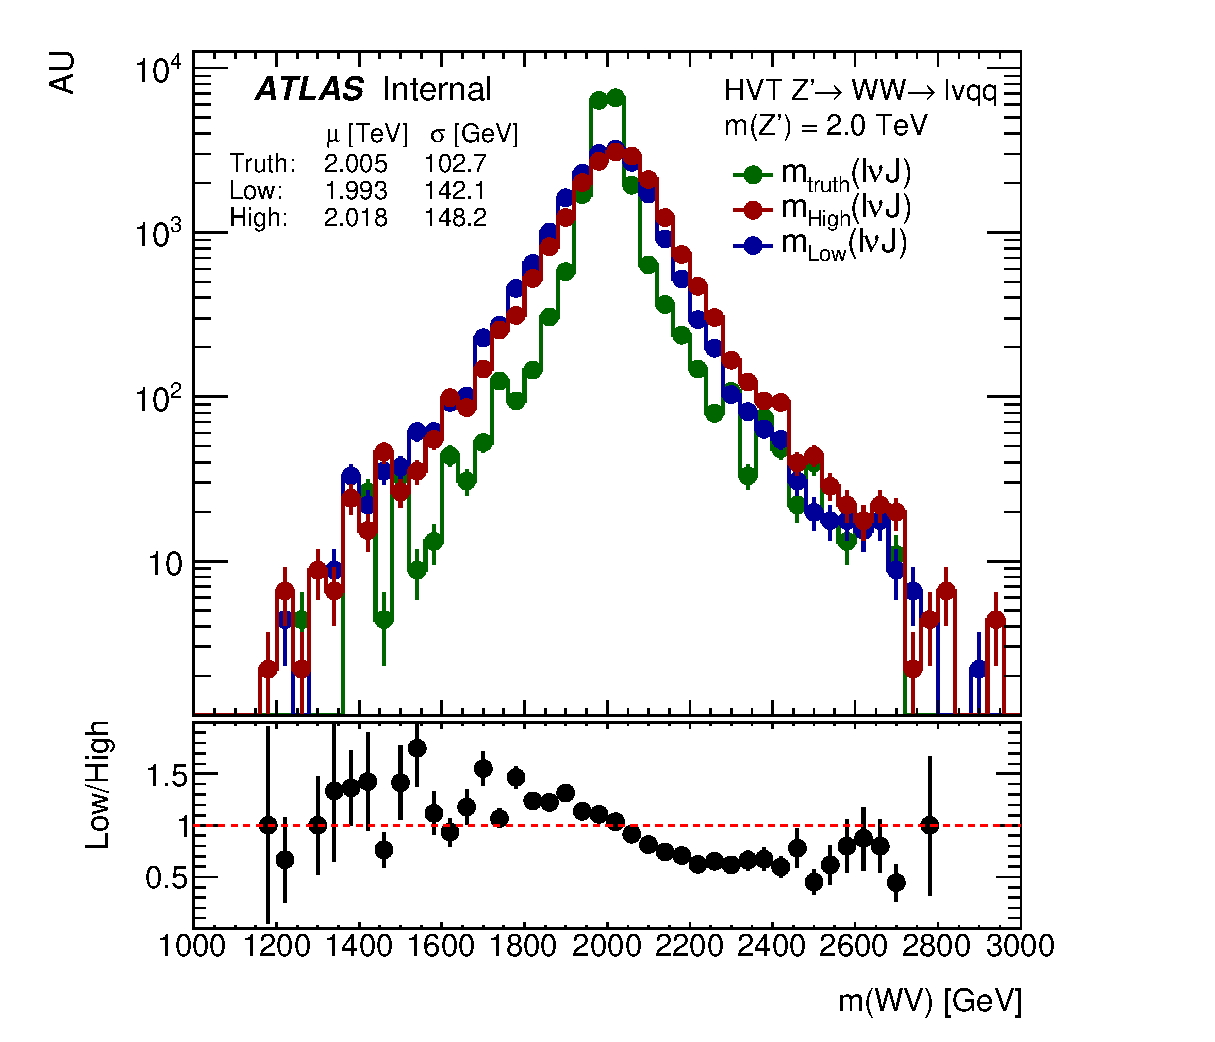
\includegraphics[width=0.49\linewidth]{figures/Appendix/h_pz_low_high}\label{fig:nz_lowhigh}}
\subfloat[]{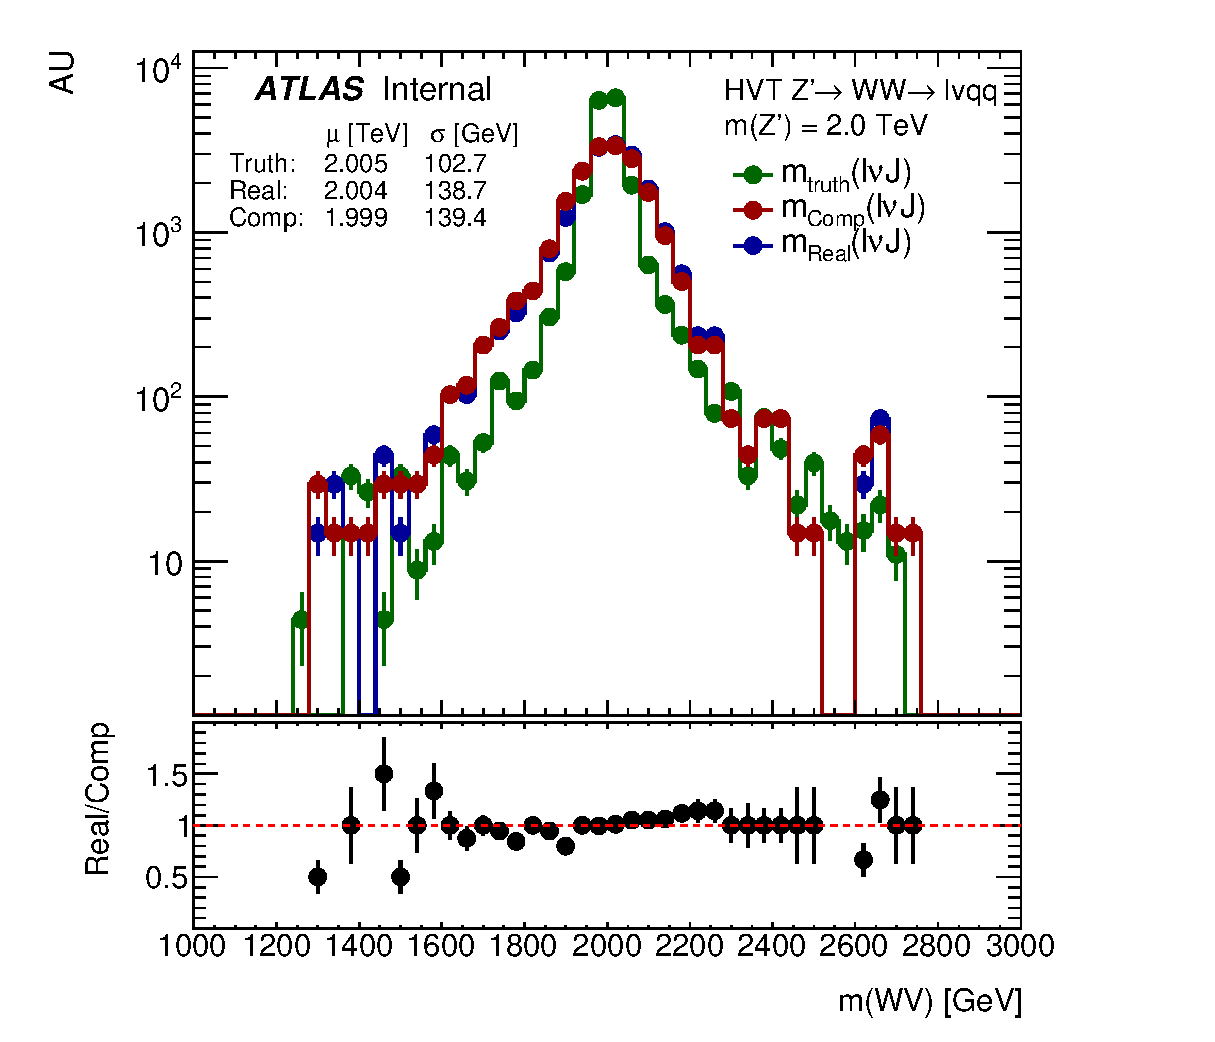
\includegraphics[width=0.49\linewidth]{figures/Appendix/h_real_complex}\label{fig:nz_realcomplex}}
\end{center}
  \caption[Neutrino $p_{z}$ solution comparisons]{The invariant mass is constructed for choice of $p_{z, \nu}$ \protect\subref{fig:nz_lowhigh} lowest (blue) vs highest (red) solution and \protect\subref{fig:nz_realcomplex} real (blue) vs complex (red) solution. The ratio (blue/red) is shown for each choice. Truth invariant mass (green) is shown as a reference.  HVT $Z'$ benchmark signal at $m=2.0\,\TeV$ is used.}
  \label{fig:neutrinoPz}
\end{figure}

\begin{figure}[hp]
  \begin{center}
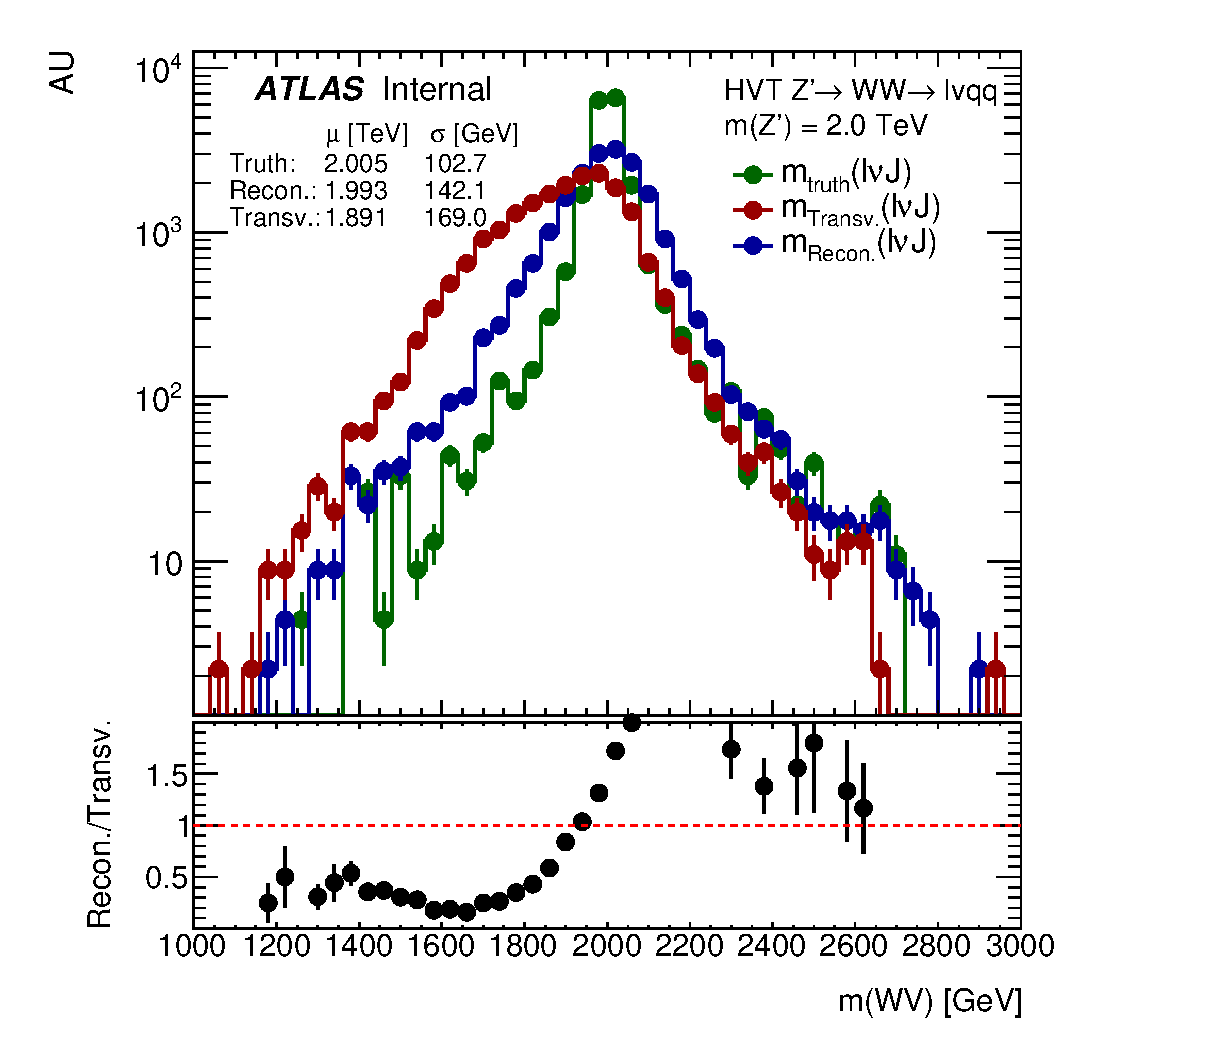
\includegraphics[width=0.6\linewidth]{figures/Appendix/h_m_mt}
     \end{center}
  \caption[Comparison between reconstructed invariant mass and reconstructed transverse mass]{The reconstructed invariant mass, $m_{WV}$ (blue), and the reconstructed transverse mass, $m_{\mathrm{T}, WV}$ (red) are shown for the HVT $Z'$ benchmark signal at $m=2.0\,\TeV$. Truth invariant mass (green) is shown as a reference. There is a significant improvement in the reconstructed mass: the peak is more centered and sharper, while the width is smaller.}
  \label{fig:mass_vs_mt}
\end{figure}



